\documentclass[12pt]{article}

\usepackage[bottom = 15mm]{geometry}
\usepackage[utf8]{inputenc}
\usepackage[T2A]{fontenc}
\usepackage[russian]{babel}
\usepackage{graphicx}
\usepackage{float}
\usepackage{caption}
\usepackage{amssymb, gensymb, amsmath}
\usepackage{mathrsfs}
\usepackage{array, colortbl}
\usepackage{multicol}


\textwidth = 16 cm
\textheight = 23  cm
\oddsidemargin = 0 pt
\topmargin = -1.5 cm
\parindent = 20 pt
\parskip = 0 pt
\flushbottom


\title{{\bf Задача 4.\,4.\,2 \\ Фазовая дифракционная решётка}}
\author{Лось Денис (группа 611)}
\date{20 мая 2018}

\begin{document}

\maketitle

\paragraph*{Цель работы: } Знакомство с работой и настройкой гониометра Г5, определение спектральных характеристик фазовой решётки(эшелета), юстировка гониометра, исследование спектра ртутной лампы для нескольких углов падения.

\paragraph*{В работе используются: } гониометр, эшелетт, ртутная лампа.

\section*{Устройство гониометра}

\begin{figure}[h!]
	\centering
	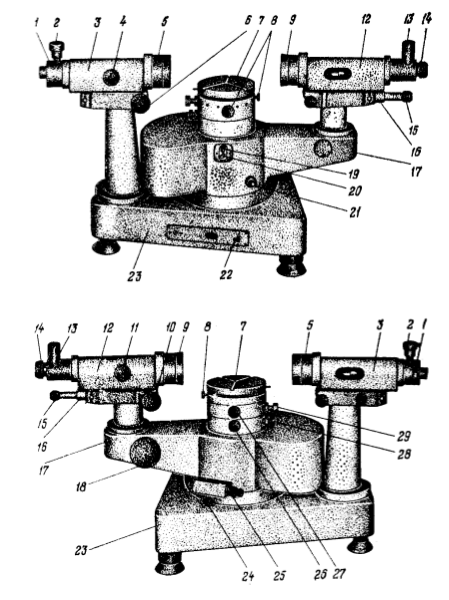
\includegraphics[width = 12cm, height = 15cm]{image1.png}
	\caption{Внешний вид гониометра}
\end{figure}
\par
	Свет от лампы Л проходит через защитную стеклянную пластинку П и попадает на автоколлимационное сетку A, содержащую две взаимно перпендикулярные щели. Свет, прошедший через сетку A, попадает на две прямоугольные призмы P и отражается от гипотенузной грани, на которую нанесён полупрозрачный слой с коэффициентом отражения $50\%$. Для юстировки гониометра на столик ставится предмет с плоской отражающей поверхностью. После отражения от неё параллельный пучок лучей возвращается назад в зрительную трубу и собирается в фокальной области объектива. В этом случае святищийся крест можно увидеть через окуляр зрительной трубы. Кроме того, в окуляре имеется ещё одна сетка С, на которой изображён чёрный отсчётный крест. Совмещённые изображения обоих крестов рассматриваются через окулярные линзы O. Резкость видимого изображения отсчётного креста регулируется вращением оправы окуляра 14.
\par
	Обе сетки окуляра, А и С, расположены на строго одинаковых расстояниях от гипотенузных граней призмы P, поэтому их одновременное наблюдение в окуляре возможно только при совпадении фокальных плоскостей объектива и окуляра (труба настроена на бесконечность).
\par
	Важнейшим узлом гониометра является устройство, служащее для отсчёта угла поворота зрительной трубы вокруг вертикальной оси, проходящей через центр столика. На этой оси крепится прозрачное кольцо, расположенное в корпусе прибора. На поверхность лимба нанесена шкала с делениями.
\par
	Оптическая система отсчётного устройства собрана так, что через окуляр можно наблюдать изображения штрихов двух диаметрально противоположных участков лимба, причём одно изображение прямое, а другое обратное. Кроме того, оптическая система позволяет перемещать эти изображения друг относительно друга, оставляя в покое как лимб, так и алидаду со зрительной трубой. Это перемещение штрихов измеряется при помощи оптического микрометра.

\section*{Качественные наблюдения}
\par
	Удерживая эшелетт в вытянутой руке, найдём отражённое изображение нити лампы накаливания, расположенной за спиной. Вращая эшелетт будем наблюдать спектры различных положительных и отрицательных порядков. Порядок, в котором наиболее интенсивен равен 1, соответствующая рабочая длина волна $\lambda_\text{б} = 500$ нм.

\section*{Исследование спектра ртутной лампы}
\par
	Установим ширину входной щели коллиматора, при которой ширина линий жёлтого дублета чуть больше промежутка между линиями двойного штриха зрительной трубы.
\par
	Для угла падения $30 \degree$ измерим угловые координаты спектральных линий ртути в рабочем порядке.
\begin{table}[h!]
	\centering
	\begin{tabular}{|c|c|c|}
	\hline
		n & $\varphi$ & цвет \\
	\hline
		3 & $294 \degree 11' 6''$ & зелёный \\
	\hline
		2 & $295 \degree 20' 25''$ & жёлтый \\
	\hline
		1 & $295 \degree 24' 52''$ & жёлтый \\
	\hline
		6 & $290 \degree 3' 26''$ & фиолетовый \\
	\hline
		5 & $292 \degree 10' 27''$ & синий \\
	\hline
		4 & $292 \degree 20' 2''$ & голубой \\
	\hline
	\end{tabular}
\end{table}
\par
	Построим график зависимости $\sin \varphi_m - \sin \psi$ от длины волны в рабочем порядке.

\begin{figure}[h!]
	\centering
	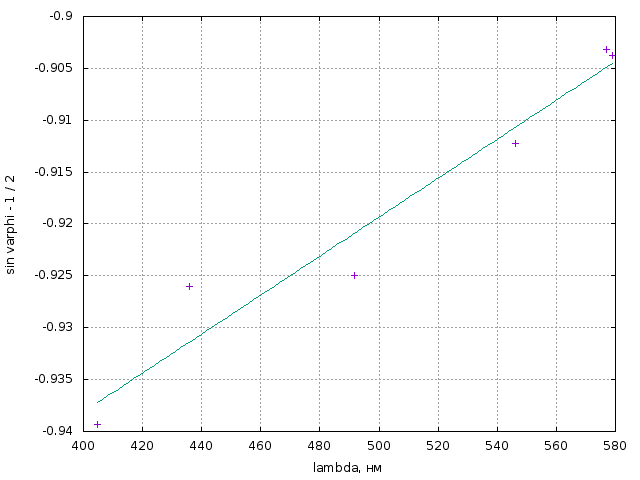
\includegraphics[width = 12cm, height = 5cm]{plot1.png}
	\caption{График зависимости $\sin \varphi_m - \sin \psi$ от $\lambda$}
\end{figure}
\par
	Коэффициент наклона графика
\[
	\beta = \left(18 \pm 3\right) \cdot 10^{-5} \, \frac{1}{\text{нм}}
\]
\par
	Тогда шаг решётки
\[
	d = \left(5.6 \pm 0.9 \right) \, \text{мкм}
\]
\par
	Определим угол скоса рабочей грани эшелетта
\[
	\sin \Omega = \frac{m_p \lambda_p}{2 d} = (0.045 \pm 0.007)
\]

\newpage
\subsection*{Определение угловой дисперсии}
\par
	Дополнительные измерения для жёлтого дуплета
\begin{table}[h!]
	\centering
	\begin{tabular}{|c|c|c|}
	\hline
		n & $\varphi$ & цвет \\
	\hline
		2 & $315 \degree 37' 7''$ & жёлтый \\
	\hline
		1 & $315 \degree 46' 10''$ & жёлтый \\
	\hline
	\end{tabular}
\end{table}

\section*{Выводы}
\par
	В ходе работы возникли сложности с настройкой и юстировкой, в результате чего достаточно большое количество времени было потрачено на предварительную работу с системой, нежели на непосредственные измерения. В результате чего было реализиовано лишь половина актуальных исследованиях. Однако стоит отметить, что в ходе этой работы былы определены шаг решётки, а также угол скоса рабочей грани эшелета.
\end{document}